\documentclass{standalone}

\usepackage{tikz}
\usepackage{amsmath, amssymb,stackrel}

%% Public TikZ libraries
\usetikzlibrary{arrows}
\usetikzlibrary{calc}
\usetikzlibrary{circuits.logic.US}
\usetikzlibrary{positioning}
\usetikzlibrary{shapes}

\DeclareMathOperator{\cor}{\mathbf{cor}}

%% Custom TikZ addons
	
%% Document

\begin{document}



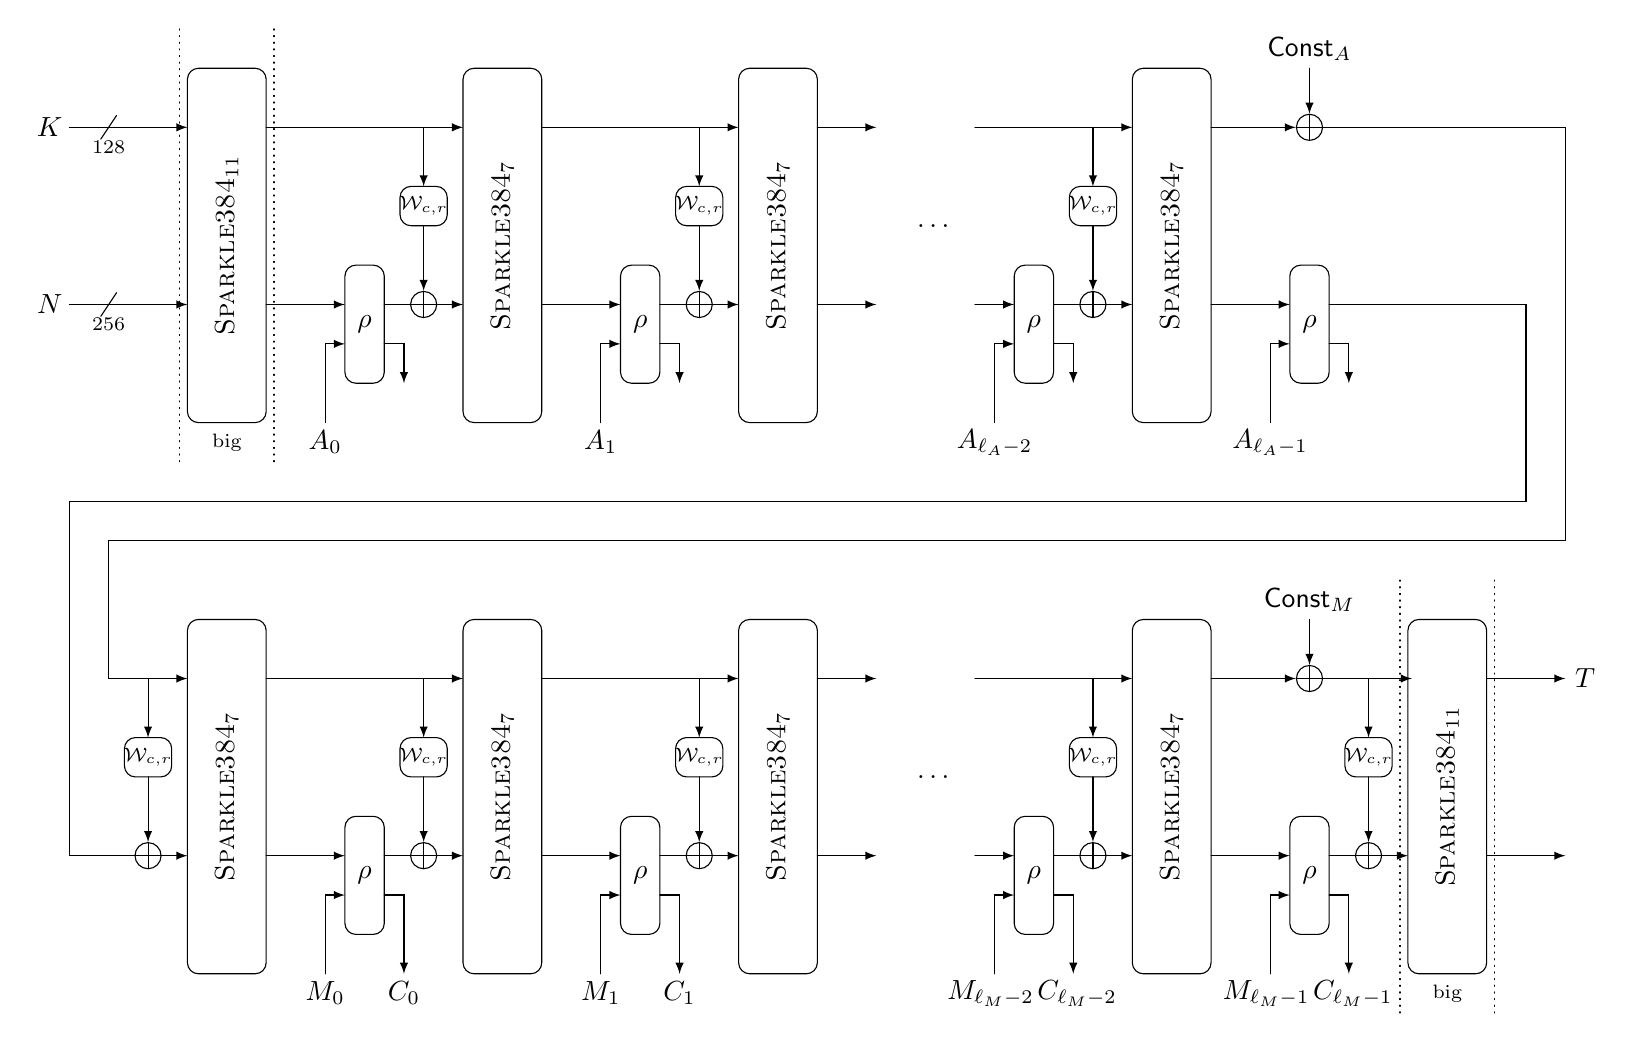
\begin{tikzpicture}[line cap=round]
\tikzset{tikzxor/.style={draw,circle,append after command={
        [shorten >=\pgflinewidth, shorten <=\pgflinewidth,]
        (\tikzlastnode.north) edge (\tikzlastnode.south)
        (\tikzlastnode.east) edge (\tikzlastnode.west)
        }
    }    
}

\tikzset{tikzadd/.style={draw,rectangle,append after command={
        [shorten >=\pgflinewidth, shorten <=\pgflinewidth,]
        (\tikzlastnode.north) edge (\tikzlastnode.south)
        (\tikzlastnode.east) edge (\tikzlastnode.west)
        }
    }   
}












\draw[rounded corners]  (-2.5,-4) rectangle (-1.5,-8.5);
\draw[rounded corners]  (1,-4) rectangle (2,-8.5);
\draw[rounded corners]  (6,-4) rectangle (7,-8.5);
%\draw[rounded corners]  (9.5,-4) rectangle (10.5,-8.5);


\draw[rounded corners] [-latex] (0,-6.5) rectangle (-0.5,-8);
\draw[rounded corners] [-latex] (5,-6.5) rectangle (4.5,-8);
\draw[rounded corners] [-latex] (8.5,-6.5) rectangle (8,-8);
\draw [-latex](-1.5,-7) -- (-0.5,-7);
\draw [-latex](0,-7) -- (1,-7);
\draw [-latex](2,-7) -- (2.75,-7);
\draw [-latex](4,-7) -- (4.5,-7);
\draw [-latex](5,-7) -- (6,-7);
\draw [-latex](7,-7) -- (8,-7);
%\draw [-latex](8.5,-7) -- (9.5,-7);
\draw [-latex](-0.75,-8.5) -- (-0.75,-7.5) -- (-0.5,-7.5);
\draw [-latex](4.25,-8.5) -- (4.25,-7.5) -- (4.5,-7.5);
\draw [-latex](7.75,-8.5) -- (7.75,-7.5) -- (8,-7.5);
\draw [-latex](0,-7.5) -- (0.25,-7.5) -- (0.25,-8);
\draw [-latex](5,-7.5) -- (5.25,-7.5) -- (5.25,-8);
\draw [-latex](8.5,-7.5) -- (8.75,-7.5) -- (8.75,-8);
\node at (3.5,-6) {$\dots$};
\draw [-latex](-1.5,-4.75) -- (1,-4.75);
\draw [-latex](2,-4.75) -- (2.75,-4.75);
\draw [-latex](4,-4.75) -- (6,-4.75);
%\draw [-latex](7,-4.75) -- (9.5,-4.75);
\draw[rounded corners] [-latex] (-6,-4) rectangle (-5,-8.5);
\draw[rounded corners] [-latex] (-4,-6.5) rectangle (-3.5,-8);
\draw [-latex](-5,-7) -- (-4,-7);
\draw [-latex](-3.5,-7) -- (-2.5,-7);
\draw [-latex](-4.25,-8.5) -- (-4.25,-7.5) -- (-4,-7.5);
\draw [-latex](-3.5,-7.5) -- (-3.25,-7.5) -- (-3.25,-8);
\draw [-latex](-5,-4.75) -- (-2.5,-4.75);
%\node[tikzxor] (v5) at (-6.75,-7) {};
%\draw [-latex](-7.5,-7) -- (v5);
%\draw [-latex](v5) -- (-6,-7);
%\draw [-latex](-6.75,-8.5) -- (v5);
\draw [-latex](-7.5,-4.75) -- (-6,-4.75);
\node[tikzxor] (v6) at (8.25,-4.75) {};
\draw [-latex](7,-4.75) -- (v6);
%\draw [-latex](v6) -- (9.5,-4.75);
\draw [-latex](8.25,-4) -- (v6);

\draw [-latex](v6) -- (11.5,-4.75) -- (11.5,-10) -- (-7,-10) -- (-7,-11.75) -- (-6,-11.75);
\draw [-latex](8.5,-7) -- (11,-7) -- (11,-9.5) -- (-7.5,-9.5) -- (-7.5,-14) -- (-6,-14);


\draw [rounded corners] (-6,-11) rectangle (-5,-15.5);
\draw [rounded corners] (-2.5,-11) rectangle (-1.5,-15.5);



\draw[rounded corners]  (1,-11) rectangle (2,-15.5);
\draw[rounded corners]  (6,-11) rectangle (7,-15.5);
\draw[rounded corners]  (9.5,-11) rectangle (10.5,-15.5);
\draw[-latex] (-5,-11.75) -- (-2.5,-11.75);
\draw [-latex](-1.5,-11.75) -- (1,-11.75);
\draw [-latex](2,-11.75) -- (2.75,-11.75);
\draw [-latex](4,-11.75) -- (6,-11.75);
\node[tikzxor] (v7) at (8.25,-11.75) {};
\draw [-latex](7,-11.75) -- (v7);
\draw [-latex](v7) -- (9.55,-11.75);

\draw[rounded corners] [-latex] (-4,-13.5) rectangle (-3.5,-15);
\draw[rounded corners] [-latex] (-0.5,-13.5) rectangle (0,-15);
\draw[rounded corners] [-latex] (4.5,-13.5) rectangle (5,-15);
\draw[rounded corners] [-latex] (8,-13.5) rectangle (8.5,-15);
\draw [-latex](-5,-14) -- (-4,-14);
\draw [-latex](-3.5,-14) -- (-2.5,-14);
\draw [-latex](-1.5,-14) -- (-0.5,-14);
\draw [-latex](0,-14) -- (1,-14);
\draw [-latex](2,-14) -- (2.75,-14);
\draw [-latex](4,-14) -- (4.5,-14);
\draw [-latex](5,-14) -- (6,-14);
\draw [-latex](7,-14) -- (8,-14);
\draw [-latex](8.5,-14) -- (9.5,-14);
\draw [-latex](-4.25,-15.5) -- (-4.25,-14.5) -- (-4,-14.5);
\draw [-latex](-0.75,-15.5) -- (-0.75,-14.5) -- (-0.5,-14.5);
\draw [-latex](4.25,-15.5) -- (4.25,-14.5) -- (4.5,-14.5);
\draw [-latex](7.75,-15.5) -- (7.75,-14.5) -- (8,-14.5);
\draw [-latex](-3.5,-14.5) -- (-3.25,-14.5) -- (-3.25,-15.5);
\draw [-latex](0,-14.5) -- (0.25,-14.5) -- (0.25,-15.5);
\draw [-latex](5,-14.5) -- (5.25,-14.5) -- (5.25,-15.5);
\draw [-latex](8.5,-14.5) -- (8.75,-14.5) -- (8.75,-15.5);
\draw [-latex](10.5,-14) -- (11.5,-14);
\draw [-latex](10.5,-11.75) -- (11.5,-11.75);
\node at (3.5,-13) {$\dots$};

\draw [-latex](8.25,-11) -- (v7);
\node[rotate=90] at (-5.5,-6.25) {$\textsc{Sparkle384}_{11}$};
\node[rotate=90] at (-2,-6.25) {$\textsc{Sparkle384}_7$};
\node[rotate=90] at (1.5,-6.25) {$\textsc{Sparkle384}_7$};
\node[rotate=90] at (6.5,-6.25) {$\textsc{Sparkle384}_7$};
%\node[rotate=90] at (10,-6.25) {$\textsc{Sparkle384}_6$};
\node[rotate=90] at (-5.5,-13.25) {$\textsc{Sparkle384}_7$};
\node[rotate=90] at (-2,-13.25) {$\textsc{Sparkle384}_7$};
\node[rotate=90] at (1.5,-13.25) {$\textsc{Sparkle384}_7$};
\node[rotate=90] at (6.5,-13.25) {$\textsc{Sparkle384}_7$};
\node[rotate=90] at (10,-13.25) {$\textsc{Sparkle384}_{11}$};
\draw [dotted](-6.1,-3.5) -- (-6.1,-9);
\draw [dotted](-4.9,-3.5) -- (-4.9,-9);
\node at (-5.5,-8.75) {\scriptsize big};
\node at (-3.75,-7.25) {$\rho$};
\node at (-0.25,-7.25) {$\rho$};
\node at (4.75,-7.25) {$\rho$};
\node at (8.25,-7.25) {$\rho$};
\node at (-3.75,-14.25) {$\rho$};
\node at (-0.25,-14.25) {$\rho$};
\node at (4.75,-14.25) {$\rho$};
\node at (8.25,-14.25) {$\rho$};
\node at (-4.25,-8.75) {$A_0$};

\node at (-0.75,-8.75) {$A_1$};
\node at (4.25,-8.75) {$A_{\ell_A-2}$};
\node at (7.75,-8.75) {$A_{\ell_A-1}$};
\node at (-4.25,-15.75) {$M_0$};
\node at (-0.75,-15.75) {$M_1$};
\node at (4.2,-15.75) {$M_{\ell_M-2}$};
\node at (7.7,-15.75) {$M_{\ell_M-1}$};



\node at (-3.25,-15.75) {$C_0$};
\node at (0.25,-15.75) {$C_1$};
\node at (5.3,-15.75) {$C_{\ell_M-2}$};
\node at (8.8,-15.75) {$C_{\ell_M-1}$};
\node at (11.75,-11.75) {$T$};
\node at (-7.75,-7) {$N$};
\node at (-7.75,-4.75) {$K$};
%\node at (-6.75,-8.75) {$N$};
\node at (8.25,-3.75) {$\mathsf{Const}_A$};
\node at (8.25,-10.75) {$\mathsf{Const}_M$};
\draw [-latex](-7.5,-7) -- (-6,-7);
\draw (-7.1,-4.9) -- (-6.9,-4.6);
\draw (-7.1,-4.9-2.25) -- (-6.9,-4.6-2.25);
\node at (-7,-5) {\scriptsize$128$};
\node at (-7,-5-2.25) {\scriptsize$256$};
%\draw [dotted](-6.25,-10.5) -- (-6.25,-16);
%\draw [dotted](-4.75,-10.5) -- (-4.75,-16);
%\node at (-5.5,-15.75) {\scriptsize separation};
\draw [dotted](9.4,-10.5) -- (9.4,-16);
\draw [dotted](10.6,-10.5) -- (10.6,-16);
\node at (10,-15.75) {\scriptsize big};
\node[tikzxor] (v1) at (-3,-7) {};

\node[tikzxor] (v9) at (0.5,-7) {};
\node[tikzxor] (v10) at (5.5,-7) {};
\node[tikzxor] (v8) at (-6.5,-14) {};
\node[tikzxor] (v5) at (-3,-14) {};
\node[tikzxor] (v4) at (0.5,-14) {};
\node[tikzxor] (v3) at (5.5,-14) {};
\node[tikzxor] (v2) at (9,-14) {};

\draw[rounded corners]  (-3.25-0.05,-5.5) rectangle (-2.75+0.05,-6);
\draw[rounded corners]  (0.25-0.05,-5.5) rectangle (0.75+0.05,-6);
\draw[rounded corners]  (5.25-0.05,-5.5) rectangle (5.75+0.05,-6);
\draw[rounded corners]  (-6.75-0.05,-12.5) rectangle (-6.25+0.05,-13);
\draw[rounded corners]  (-3.25-0.05,-12.5) rectangle (-2.75+0.05,-13);
\draw[rounded corners]  (0.25-0.05,-12.5) rectangle (0.75+0.05,-13);
\draw[rounded corners]  (5.25-0.05,-12.5) rectangle (5.75+0.05,-13);
\draw[rounded corners]  (8.75-0.05,-12.5) rectangle (9.25+0.05,-13);
\node at (-3,-5.75) {\scriptsize$\mathcal{W}_{c,r}$};
\node at (0.5,-5.75) {\scriptsize$\mathcal{W}_{c,r}$};
\node at (5.5,-5.75) {\scriptsize$\mathcal{W}_{c,r}$};
\node at (-6.5,-12.75) {\scriptsize$\mathcal{W}_{c,r}$};
\node at (-3,-12.75) {\scriptsize$\mathcal{W}_{c,r}$};
\node at (0.5,-12.75) {\scriptsize$\mathcal{W}_{c,r}$};
\node at (5.5,-12.75) {\scriptsize$\mathcal{W}_{c,r}$};
\node at (9,-12.75) {\scriptsize$\mathcal{W}_{c,r}$};
\draw [-latex](-3,-4.75) -- (-3,-5.5);
\draw [-latex](-3,-6) -- (v1);
\draw [-latex](0.5,-4.75) -- (0.5,-5.5);
\draw [-latex](0.5,-6) -- (v9);
\draw [-latex](5.5,-4.75) -- (5.5,-5.5);
\draw [-latex](5.5,-6) -- (v10);
\draw [-latex](-6.5,-11.75) -- (-6.5,-12.5);
\draw [-latex](-6.5,-13) -- (v8);
\draw [-latex](-3,-11.75) -- (-3,-12.5);
\draw [-latex](-3,-13) -- (v5);
\draw [-latex](0.5,-11.75) -- (0.5,-12.5);
\draw [-latex](0.5,-13) -- (v4);
\draw [-latex](5.5,-11.75) -- (5.5,-12.5);
\draw [-latex](5.5,-13) -- (v3);
\draw [-latex](9,-11.75) -- (9,-12.5);
\draw [-latex](9,-13) -- (v2);
\end{tikzpicture}
\end{document}
